\section{The editor aspect}
\label{chap:editor_aspect}
After we have imported all concepts, their contents (properties) and linked them together (child links), it is time to define, what is the visual representation of these concepts.
Without this, we are not able to start using the language inside MPS.
\\

As stated before (section~\ref{chap:about_editor_aspect}), MPS uses a cellular system, that allows placing concept's properties and children into a table-like arrangement.
MPS has a lot of a different types of cells, that we can use:

\begin{itemize}
	\item Cells for storing values of properties -- user can enter text inside, which is validated using the type of the property (think XML tag name).
	
	\item Cells for storing child concepts -- here we can store other parser rule references and build the AST further.
	
	\item Cells that have static fixed content, such as constant keyword -- we will use these to display literal elements.
	
	\item Cells that alter the layout, such as indenting -- these dictate the layout, which we also care about.
\end{itemize}

Our import plugin has to create these cells and ideally project all of concept's elements in there.
\\

A part of this thesis' mission was to explore, whether we can also bring some more value into this import step.
The problem with grammars is, that it serves us no aid when it comes to element layout.
The grammar only defines, what the rule breaks up into and which elements (rule references, literals..) are contained inside of each alternative.
We will look into the problem of creating this missing information, either with users help or using some heuristics.
It is a very hard problem though, since our plugin doesn't really understand the contents of the grammar on some higher level.

\subsection{The interactive approach}

Since the layout information is just missing, we decided to ask the user for it.
First idea on how to tackle this problem, was to interactively prompt the user during the import process.
We would somehow select rules, that we consider important, and give the user several visual options on how we think this rule might be laid out.
The user would pick one and we would use this information to create the editor aspect.
There are some problems with this though, that led the author to rejecting this approach.

\subsubsection{Detecting interesting rules}

Firstly, we would have to be able to tell, which rules might be worth "discussing" with the user.
\\

The first idea for a heuristic indicating these "interesting" rules was based on number of elements contained in rule's alternative.
For simple rules, which there usually is a big number present in the grammar, we would skip them.
For complex rules (let's say 5 elements and more), we would ask the user for help with the layout.
The heuristics isn't bad, it would detect complicated rules, such as cycles, branching commands and so on, so it might be a sufficient, yet simple, solution.
It, however, has some problems --- rules describing a block of statements are usually very simple, example given being the JavaScript one:

\begin{antlr}
	\parserrule{statementList} : \parserrule{statement}* ;
\end{antlr}

This rule would be skipped by our heuristics, since the alternative has only one element, but in most general purpose languages, this is exactly the kind of statement, that we would like to alter, since normally we put each statement on a separate line.
There are dozens of rules, that have this form though (method parameters, operands, ...), and we have no means of recognizing, that this particular one should be a vertical list (meaning its elements should be separated with a new line).
\\

Another heuristics suggestion was detecting pair symbols among alternative's literal elements.
Usually, characters such as braces are a good indicator of some indenting.
We, however, did not implement any of these heuristics, because in the end, we decided to abandon the interactive approach completely, as described below in \ref{chap:interactive_approach_evaluation}.
That is why, we will not go into more detail here.

\subsubsection{Fixing rule layout}

Once we have detected a rule, that might have some interesting layout, we would ask the user to help us with it.
Consider, for example, the first alternative of the \parserrule{element} rule from the XML language:

\begin{antlr}
	\parserrule{element}  :   \literal{<} \lexerrule{Name} \parserrule{attribute}* \literal{>} \parserrule{content}* \literal{</} \lexerrule{Name} \literal{>} ;
\end{antlr}

Let's say, we would prepare few versions of how we think the layout could look like.
We could ask the user, whether attributes should be spread out horizontally or each on a new line.
We could and probably would have to do this for each element, since the plugin has no real understandind of the content.
We would have to ask for identation, line breaks etc. and we would probably not guess right, since there are just too many options.
The user would probably end up finalizing the layout himself.
\\

The other option would be some even more sophisticated interactive approach, where the user would drag the elements around or position them through some text field.
Again, we are not going into any more detail, as this approach was rejected.

\subsubsection{Approach evaluation}
\label{chap:interactive_approach_evaluation}

The author of this thesis came to a conclusion, that the results of the interactive approach would be most likely quite suboptimal.
It would be hard to recognize rules, that are in need of a refactoring.
Furthermore, when asking for users help, we would just duplicate the functionality of MPS's built in editor of the projectional editor aspect.
We would hardly mimic all of its functionality and put a lot of effort into something already existent.
Our end user is expected to have knowledge of the MPS editor, since he is importing language there.
This means, that he probably knows his way around the projectional editor too.
It wouldn't make sense to force the user to learn working with our own interactive dialog, while in background, this dialog would be just translating the layout back into the terms of the projectional editor.

\subsection{The learning approach [TODO]}

The second approach is more complex and might yield better results, we have however not implemented it, as we met some obstacles.
We would like to describe it anyway, so possible follow-up work might take it into consideration.

\subsection{Our solution [TODO]}
\label{chap:editor_solution}

\textbf{[TODO navazat na predchozi kapitolu, ted jsme to vytrhli]}
When the author of this thesis worked on the plugin, he noticed, that the most tiresome and probably error prone part of working on the editor aspect is incorporating all concept's properties, children and constant fields into the editor.
This is the phase, that takes a lot of time when building MPS languages, but does not require any major thought on user's part.
The author has further noticed, that when the plugin would do this heavy lifting in any simple way, such as plain inlining all of the cells in a single row, further adjustment of the editor is very fast, since MPS offers clever intentions and menus that enable to do this very conveniently.
In figure \ref{fig:editor_adjustment}, we can see editor adjustment of the \concept{Element{\_}1} concept.
\\

\begin{figure}[h]
	\centering
	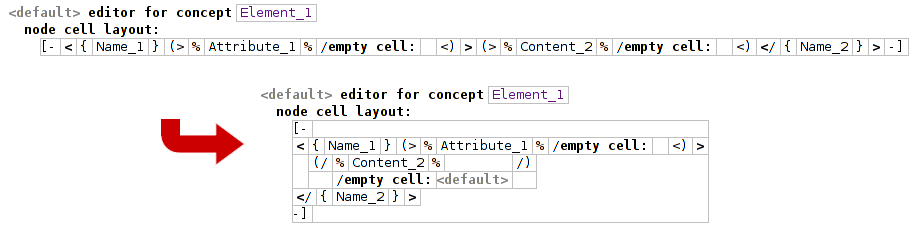
\includegraphics[width=\textwidth]{./img/editor_adjustment.png}
	\caption{Projectional editor adjustment of the Element{\_}1 concept}
	\label{fig:editor_adjustment}
\end{figure}

From these reasons, we concluded, that it is sufficient, if the plugin would only prepare contents of all editor aspects and the end user would take it from there.
We have confirmed this assumption by importing the JavaScript language~\cite{javascript} and manually adjusting all editors, that needed it, in a less than hour time.

